\section{Safety}
\label{cha:Safety}

\textbf{Read this chapter carefully before installation and use of the instrument.}

\subsection{Introduction}
Adjustment, maintenance and repair of the exposed equipment shall be carried out only by qualified personnel who are aware of hazards involved.

\subsection{Safety Precautions}
For the correct and safe use of the instrument, it is essential that both operating and servicing personnel follow generally accepted safety procedures in addition to the safety precautions specified in this manual. Specific warning and caution statements, where applicable, are found throughout this manual. Note that warning and caution statements and/or symbols are marked on the instrument as well. This manual provides technical information important for safe operation of the equipment. Please refer to the relevant sections of the manual for technical specifications, installation and
operating instructions. 

Special attention must be paid to the following issues:

\begin{itemize}
\item[-] Protective earthing of the instrument is required for the accessible terminals to be safe. (IEC 1010-1 Safety class I instrument)
%
\item[-] The actual environmental conditions must be checked against the specification.
\item[-] Mains voltage must be inside the specified range.
\end{itemize}

\subsection{Use of Caution and Warning Statements}

\paragraph{Caution}

Used to indicate correct operation or maintenance in order to prevent damage to, or destruction of equipment or other property.

\paragraph{Warning}

Used to indicate a potential hazard that requires correct procedures or practices in order to prevent personal injury.

\subsection{Symbols}
\begin{tabular}{l|l}
	\hline
	\textbf{Symbol:} & \textbf{Explanation:} \\
	\hline
	& \\
	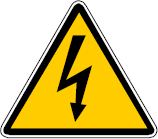
\includegraphics[width=2em]{fig/hazard} & Caution, risk of electric shock\\
	
\includegraphics[width=2em]{fig/caution} & Caution (refer to accompanying documents)\\
	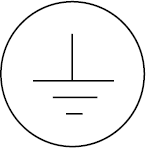
\includegraphics[width=2em]{fig/ground_symbol} & Protective conductor terminal\\
	
\includegraphics[width=2em]{fig/AC_symbol} & Alternating current\\
%	\multirow{3}{*}{
\includegraphics[width=2em]{fig/on_off_switch}} 	& Off (supply - mains switch)\\
%																																		&														\\
%																																		& On (supply - mains switch)\\
\end{tabular}

\subsection{Impaired Safety Protection}

Whenever it is likely that safe operation is impaired, the instrument must be made inoperative and secured against unintended operation. The appropriate servicing authority must be informed. For example, safety is likely to be impaired if the instrument fails to perform the intended functions or shows visible damage.

\begin{center}
\fbox{
\parbox{0.95\textwidth}{
\textbf{WARNING}: Protection provided by the equipment may be impaired, if the equipment is used in a manner not specified by this manual.
}}
\end{center}

\subsection{Technical Assistance}
Technical assistance may be obtained from your local DK-Technologies customer support organization or from:

\begin{tabular}{@{}l}
{\large DK-Technologies A/S }\\
Marielundvej 37D\\
DK-2730 Herlev\\
Denmark\\
\end{tabular}

\begin{tabular}{@{}l l}
Phone: & +45 4485 0255\\
Fax: & +45 4485 0250\\
E-Mail: & info@dk-technologies.com\\
Website: & \href{http://www.dk-technologies.com}{http://www.dk-technologies.com/}\\
\end{tabular}